\documentclass[runningheads]{llncs}

\usepackage{graphicx}
\usepackage{todonotes}
\usepackage{listingsutf8}
\usepackage[hidelinks]{hyperref}
\usepackage{cleveref}

\renewcommand\UrlFont{\color{blue}\rmfamily}

\begin{document}

\title{CaRSA Data Identify, Collect, and Connect: A second-generation, national GeoLD system in Australia}
\titlerunning{CaRSA LocI}

\author{
    Nicholas J. Car\inst{1}\orcidID{0000-0002-8742-7730} \and \\
    Irina Bastrakova\inst{2}
}

\authorrunning{Car N.J. et al.}

\institute{
    {
    SURROUND Australia Pty Ltd., Australia \&\\
    Australian National University, Australia\\
    \email{nicholas.car@surroundaustralia.com}
    %\url{https://surroundaustralia.com}
    }
    \and
    {
        Geoscience Australia\\
        \email{irina.bastrakova@ga.gov.au}
    }
}

\maketitle

\begin{abstract}
In 2018 – 2020, Australia built two \textit{Linked Data} ``spines'' - themed collections of interoperable reference data - called LocI and LongSpine. 
LocI (Location Index) consists of 7 nationally-significant spatial datasets such as the Australian Statistical Geographies System. 
LongSpine (Longitudinal Spine of Government Functions) consists of multiple datasets of Australian government structure, such as the 
Australian Government Organisations Register, as well as vocabularies of government functions. Both projects interpreted existing open 
datasets into Linked Data form and provided online delivery of their the parts as well as infrastructure for their use as a single system.\\

Here described is the Climate and Resilience Services Australia’s Data Identify, Collect and Connect project's next-generation 
implementation of the ``spines'' patterns and architecture and partial direct reuse of LocI. We discuss: differences with the originals, in particular LocI; original 
element reuse; and future-proofing steps, technical and non-technical. We also discuss the new expectations placed on this second-generation 
system, in particular the requirement to work with non-Linked Data spatial data systems, and how this system 
is pushing spatial and \textit{Semantic Web} standards development such as DGGS and GeoSPARQL.

\keywords{Location Index \and LocI \and LongSpine \and GeoSPARQL \and DGGS \and Spatial Data on the Web \and Australia \and data spine \and national data infrastructure}
\end{abstract}


\section{Introduction}\label{sec:introduction}
\subsection{CaRSA Motivation}
Climate and Resilience Services Australia (CaRSA) is a new Australia government cross-agency initiative\footnote{``Australia commits to climate resilience'', \url{https://minister.awe.gov.au/ley/media-releases/australia-commits-climate-resilience}}
that will:

\begin{quote}
    connect and leverage the Commonwealth’s extensive climate and natural disaster risk information to further prepare for and build 
    resilience to natural disasters
\end{quote}

Since Australia is prone to very damaging natural disasters such as bush fires, floods and droughts, this is a major government initiative
allocated good resourcing and the commitment is for multiple years.

\subsection{CaRSA Demonstrator Projects}
Several of the demonstrator projects for CaRSA sought to test different ways of combining information from multiple government agencies 
relevant to natural disaster management. Traditional methods of data aggregation are being tested, such as data pooling in shared facilities,
standardiseing web service-delivered information and cross-cataloging datasets, but forward-looking methdos are too. In particular,
\textit{Semantic Web} (SW) and \textit{Linked Data} (LD) technologies\footnote{By ``Linked Data'', as opposed to ``linked data'' or ``data linkage'' etc.,
we mean systems and data that implement a number of \textit{Semantic Web} technologies (RDF, OWL, SKOS, SPARQL, etc.) which are primarily 
defined as a series of \href{https://www.w3.org/standards/semanticweb/data}{World Wide Web Consortium} (W3C) standards. The W3C's defintion of 
\textit{Semantic Web} is that it is a ``Web of Data'', an evolved Internet able to be queried by machineswhich can draw inferences from it.}
are being used to integrate different, but relativley similar, datasets that are published in a distributed manner and
\textit{Discrete Global Grid System} (DGGS) spatial data methods are being used to integrate spatial data from multiple sources.

This paper describes the SW/LD and DGGS approaches being implemented in CaRSA's ``Data Identify, Collect, and Connect'' project that we will 
refere to as \textit{the project}. The project extends the approach taken by the Location Index project described in the next section.

\section{LocI: The Loction Index}\label{sec:loci}

\begin{figure}[htb]
    \centering
    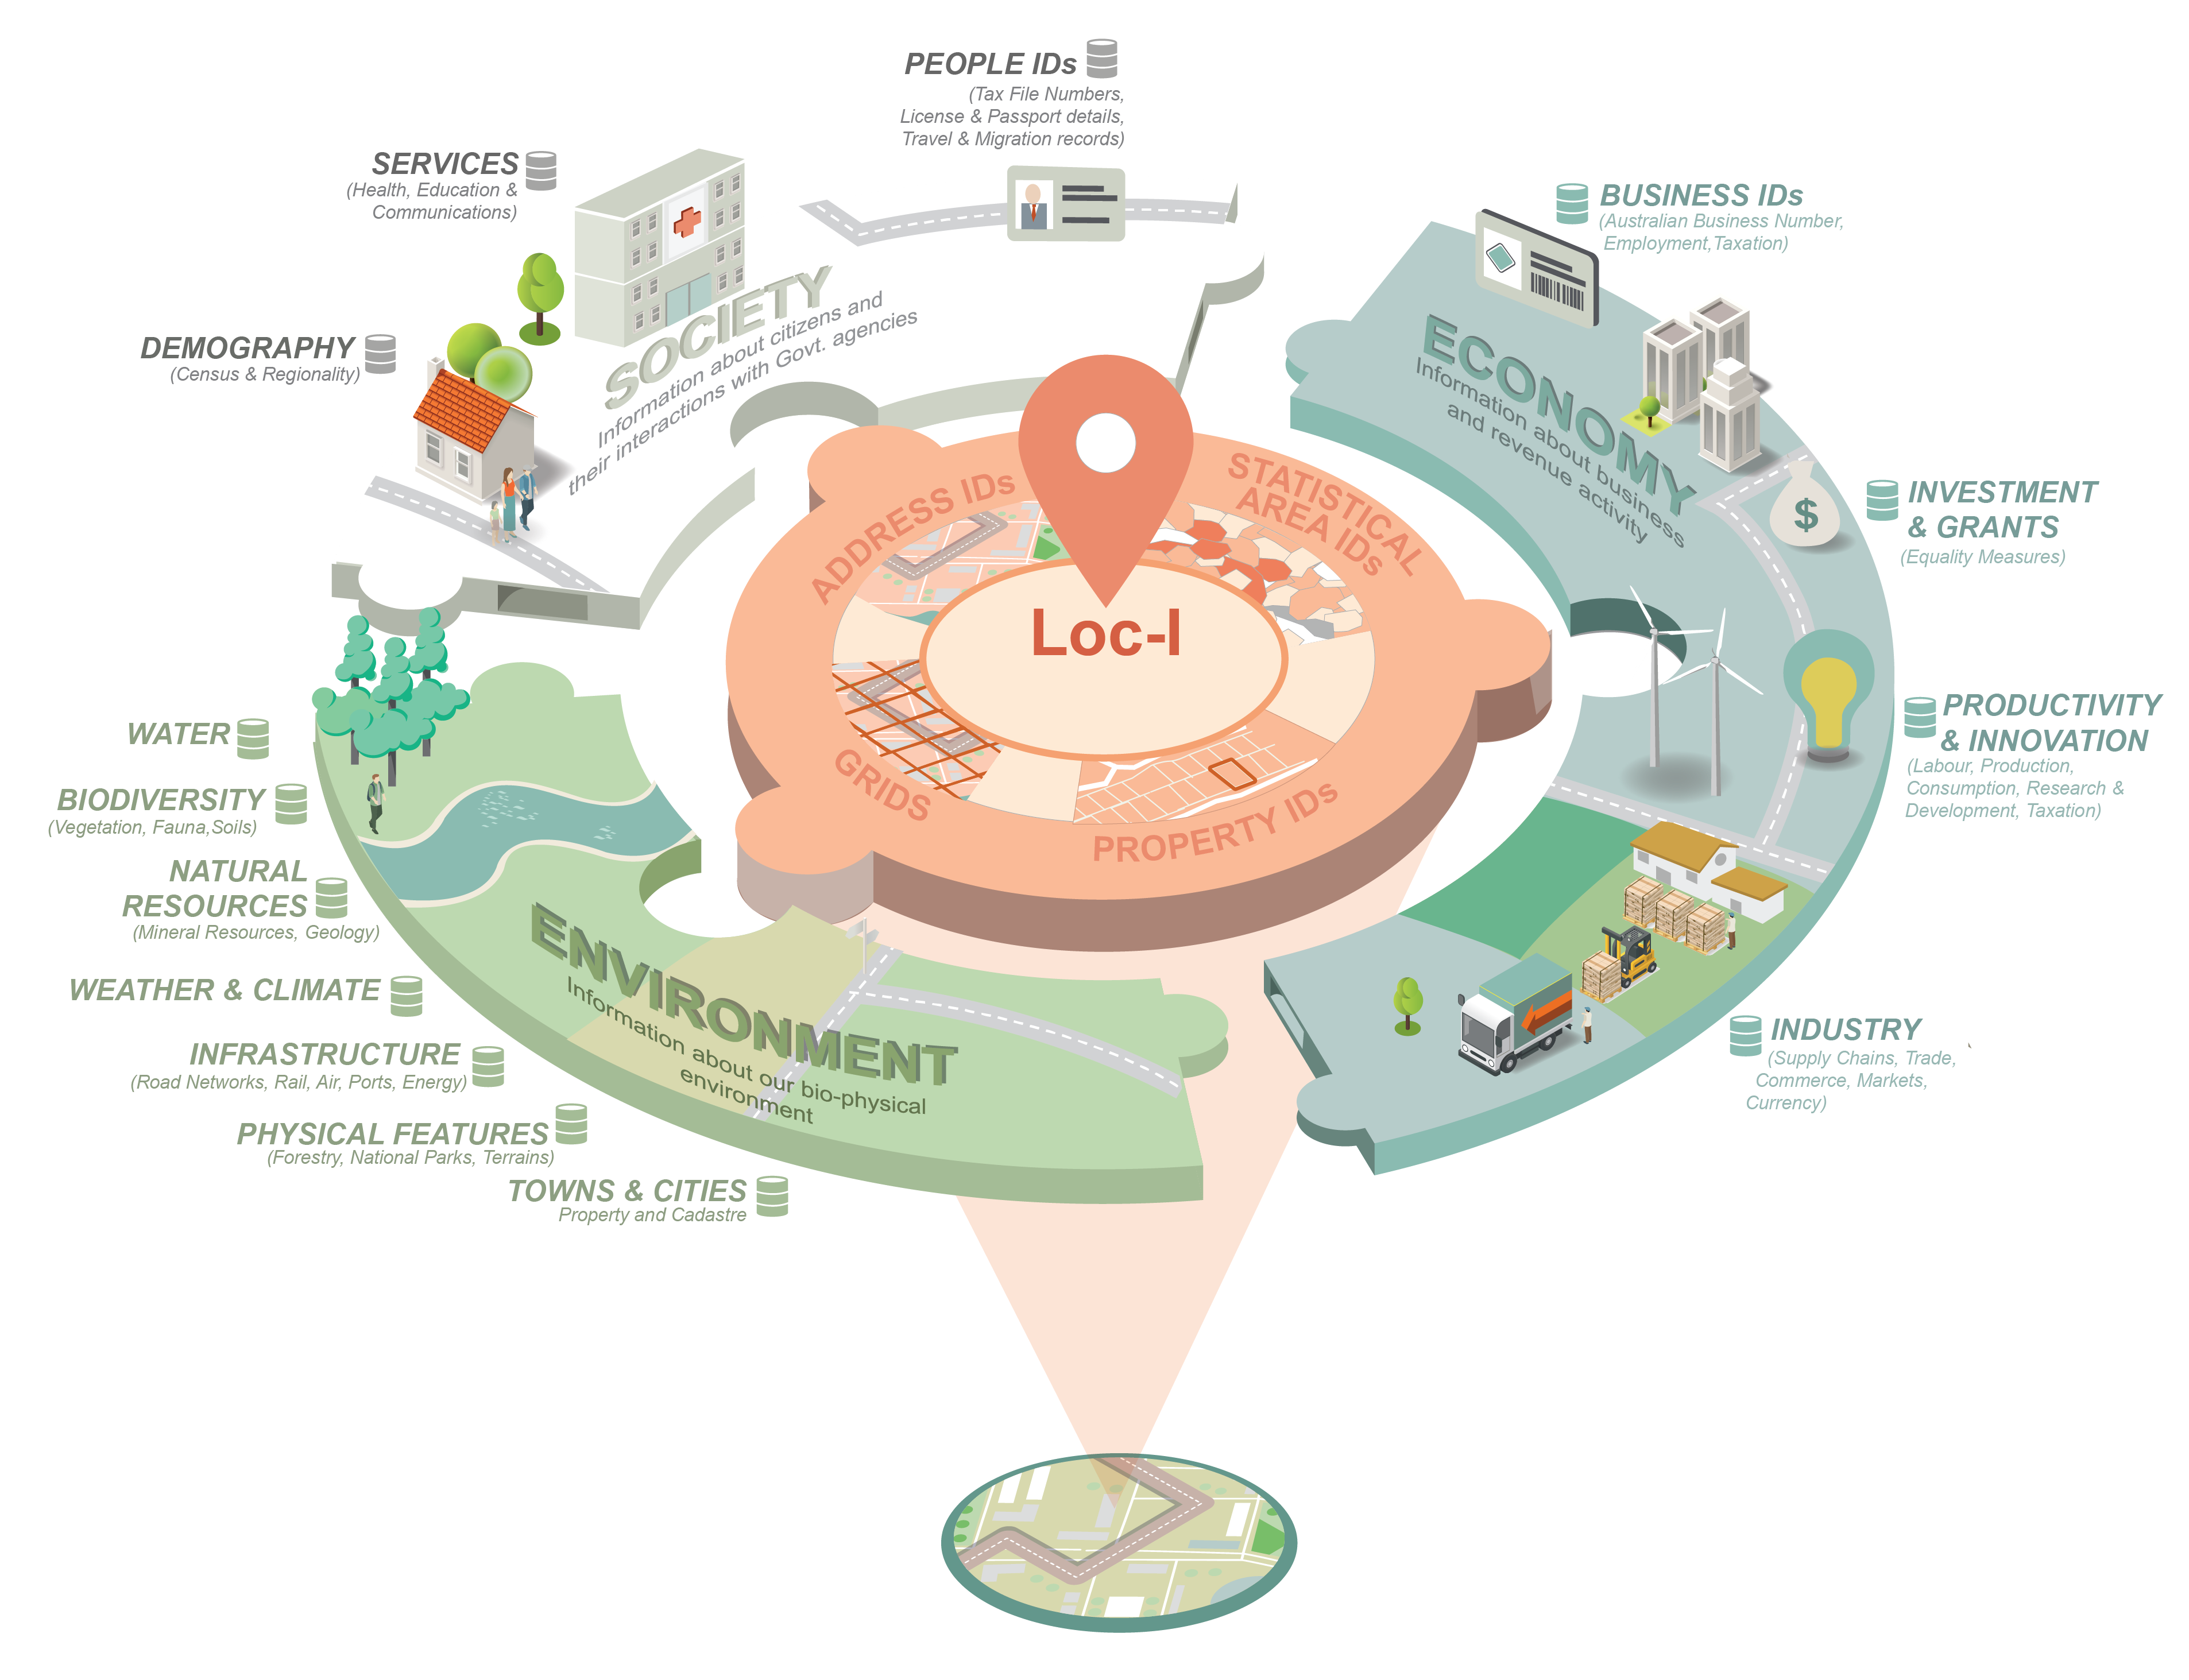
\includegraphics[width=\linewidth]{images/loci-brochure.png}
    \caption{A project brochure image, from \cite{car_location_2019}, of LocI with respect to
    Australian government \textit{Environment}, \textit{Society} and \textit{Economy} data}
    \label{fig:geosparql11ontology}
\end{figure}

In 2018 - 2020, Australian spatial data and research agencies implemented a:

\begin{quotation}
    national and authoritative, also federated, index for Australian spatial data using Semantic Web technologies~\cite{car_location_2019}
\end{quotation}

This system, known as the Location Index (LocI)~\cite{car_location_2019}, aims to ``better geospatially integrate and analyze data across 
government portfolios and information domains''. The main use case addressed by LocI's is to greatly reduce the time taken by government 
workers in data analysis using spatial information by providing pre-integrated, authoratitive, spatial datasets that can be used in 
online, open data scenarios, within secure data integration environments and across the two.

Some of the interesting aspects of LocI's design include:

\begin{itemize}
    \item[$\ast$] federated publication of datasets via standard Linked Data APIs
    \item[$\ast$] use of VoID \texttt{Linkset}~\cite{alexander_describing_2011} instances to crosswalk datasets
    \begin{itemize}
        \item[$-$] these are independently-selectable for use meaning that a specific ccrosswalk, of potentially many, may be selected for use
    \end{itemize} 
    \item[$\ast$] use of a \textit{Geometry Data Service}\footnote{The service is online at \url{https://gds.loci.cat/}} for spatial integration
    \begin{itemize}
        \item[$-$] this service extends common use of using GeoSPARQL~\cite{open2012ogc} by storing \texttt{Geometry} instances seperately from the \texttt{Feature} instances they are the geometries for. This allows the geometry data to be managed in a PostGIS database~\footnote{\url{https://postgis.net/}}, not a triplestore, as usually used for GeoSPARQL data.
    \end{itemize}
    \item[$\ast$] several different clients for different uses
    \begin{itemize}
        \item[$-$] such as \textit{Excelerator}\footnote{\url{https://loci.cat/excelerator.html}}, used to upload data according to one spatial reference system and download it reapportioned according to another
    \end{itemize}
\end{itemize} 

LocI's initial spatial datasets are from a number of domains including environmental (the \textit{Australian Hydrological Geospatial Fabric}
\footnote{The original, non-RDF dataset: \url{http://www.bom.gov.au/water/geofabric/}, and the online LD version implemented by LocI: \url{http://linked.data.gov.au/dataset/geofabric}}, 
a collection of surface hydrology features), human/census (the \textit{Australian Statistical Geography Standard} spatial areas)
\footnote{Non-RDF dataset: \url{https://geo.abs.gov.au/arcgis/services/ASGS2016/MB/MapServer/WFSServer}, LD version: \url{http://linked.data.gov.au/dataset/asgs2016}}, 
and cartographic/administrative (the \textit{National Composite Gazetteer of Australia})\footnote{LD version: \url{https://linked.data.gov.au/dataset/placenames}}. 

The LocI system's architecture is shown in \ref{fig:loci-arch} for architectural details. It shows the LocI Data Cache, which is a multi-graph triplestore, 
obtains its data by ``pulling'' RDF datasets through APIs that both interpret non-RDF data for online delivery and are also able to create static RDF 
versions of the datasets. All LocI datasets conform to the LocI Ontology\footnote{\url{http://linked.data.gov.au/def/loci}} which imports the GeoSPARQL
\footnote{\url{http://www.opengis.net/doc/IS/geosparql/1.0}} and DCAT\footnote{\url{https://www.w3.org/TR/2014/REC-vocab-dcat-20140116/}} ontologies. 
Alongside the Cache is a traditional spatial DB - PostGIS\footnote{\url{https://postgis.net/}} used to perform fast geometry intersections.

\begin{figure}[htb]
    \centering
    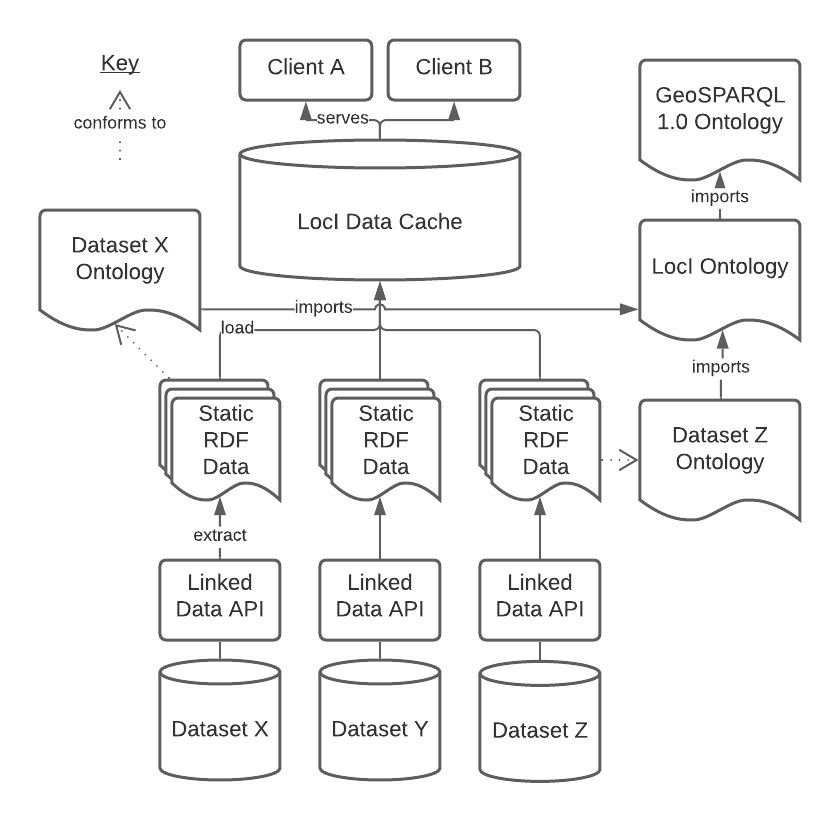
\includegraphics[width=\linewidth]{images/loci-arch.png}
    \caption{An informal architecture diagram of the LocI project's \textit{Linked Data} infrastructure.}
    \label{fig:loci-arch}
\end{figure}

\section{CaRSA Project Changes}\label{sec:changes}




\begin{figure}[htb]
    \centering
    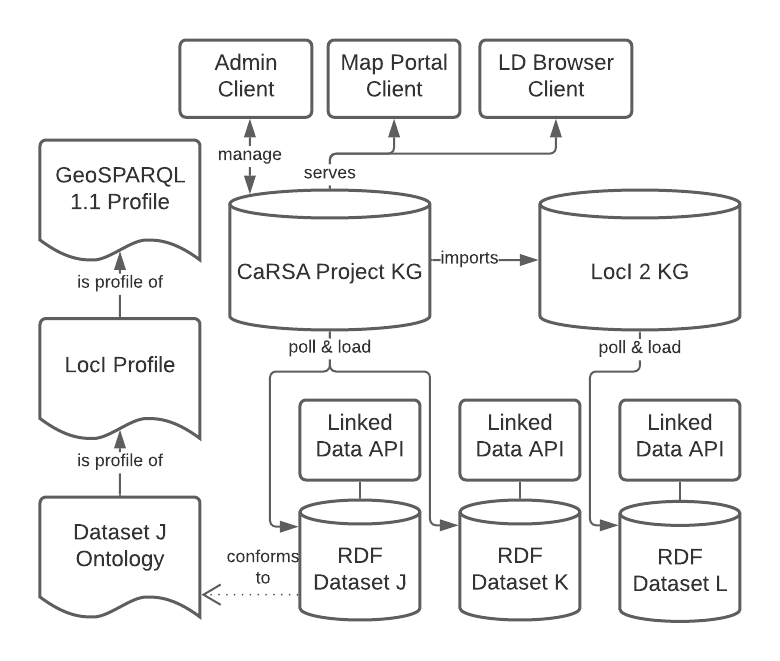
\includegraphics[width=\linewidth]{images/carsa-arch.png}
    \caption{An informal architecture diagram of the CaRSA project's \textit{Linked Data} infrastructure}
    \label{fig:geosparql11ontology}
\end{figure}


\section{Conclusions}\label{sec:conclusions}




\subsection{Future Work}\label{sec:futurework}
\begin{itemize}
    \item[$\ast$] GeoSPARQL 1.1: to be completed by July, 2021
    \item[$\ast$] GeoSPARQL 1.2: more adventurous extension - late 2021
    \item[$\ast$] GeoSPARQL 2.0: so-far unspecified
\end{itemize}


%
% ---- Bibliography ----
%
% BibTeX users should specify bibliography style 'splncs04'.
% References will then be sorted and formatted in the correct style.
%
\bibliographystyle{splncs04}
\bibliography{references}
%
% \begin{thebibliography}{8}
% \bibitem{ref_article1}
% Author, F.: Article title. Journal \textbf{2}(5), 99--110 (2016)

% \bibitem{ref_lncs1}
% Author, F., Author, S.: Title of a proceedings paper. In: Editor,
% F., Editor, S. (eds.) CONFERENCE 2016, LNCS, vol. 9999, pp. 1--13.
% Springer, Heidelberg (2016). \doi{10.10007/1234567890}

% \bibitem{ref_book1}
% Author, F., Author, S., Author, T.: Book title. 2nd edn. Publisher,
% Location (1999)

% \bibitem{ref_proc1}
% Author, A.-B.: Contribution title. In: 9th International Proceedings
% on Proceedings, pp. 1--2. Publisher, Location (2010)

% \bibitem{ref_url1}
% LNCS Homepage, \url{http://www.springer.com/lncs}. Last accessed 4
% Oct 2017
% \end{thebibliography}
\end{document}




% Outline
% 
% Section 1
%   History of GeoSPARWL 1.0
% Section 2
%   motivation to update the spec
% Section 3
%   GeoSPARQL 1.1 additions
%       motivation, and expected use, of new spatial functions. In particular, why in GeoSPARQL when aggregations etc. can be performed elsewhere?
%       Spatial Measure
% Section 4
%       new profile presentation
%       new URI regimes etc
% Section 5
%       expected changed use modes